% 2024年北京高考数学第8题：四棱锥P-ABCD
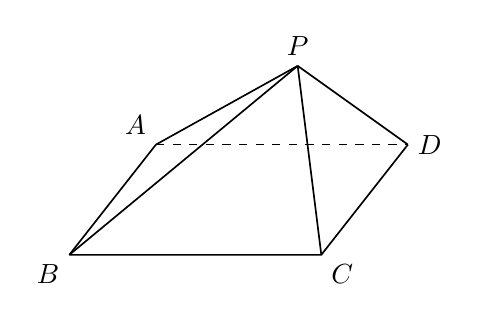
\begin{tikzpicture}[>=stealth,line width=0.6pt,font=\normalsize]
  \coordinate (B) at (0,0);
  \coordinate (C) at (3.2,0);
  \coordinate (D) at (4.3,1.4);
  \coordinate (A) at (1.1,1.4);
  \coordinate (P) at (2.9,2.4);

  % 实线可见边
  \draw (B) -- (C) -- (D);
  \draw (B) -- (A);
  \draw (P) -- (B);
  \draw (P) -- (C);
  \draw (P) -- (D);
  \draw (P) -- (A);

  % 虚线不可见底边
  \draw[dashed] (A) -- (D);

  % 顶点标注
  \node[above] at (P) {$P$};
  \node[above left] at (A) {$A$};
  \node[below left] at (B) {$B$};
  \node[below right] at (C) {$C$};
  \node[right] at (D) {$D$};
\end{tikzpicture}
